\section{Konzept 1}

\begin{figure}[h!]
	\centering
	\begin{subfigure}[b]{0.45\textwidth}
		\includegraphics[width=\textwidth]{../../fig/Drehrad_Mitnehmer.jpg}
		\caption{Drehrad mit Mitnehmer}
	\end{subfigure}
	\begin{subfigure}[b]{0.45\textwidth}
		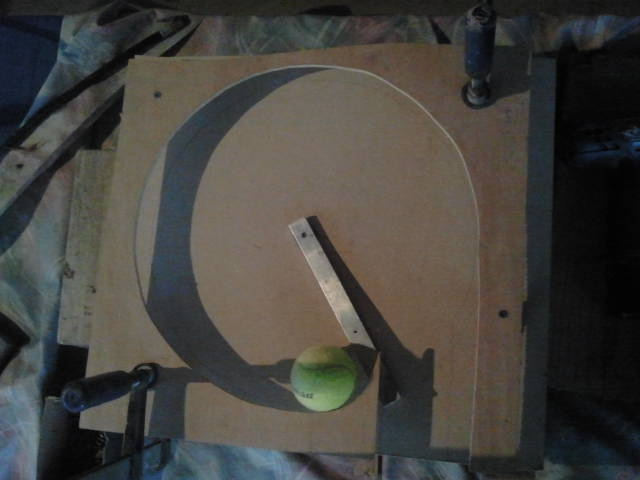
\includegraphics[width=\textwidth]{../../fig/prototyp_propeller.jpg}
		\caption{Prototyp Drehrad mit Mitnehmer}
	\end{subfigure}
	\caption{Testaufbau}
	\label{fig:drehrad_mitnehmer}
\end{figure}

\subsection{Idee}
Bei dieser Variante werden die Tennisbälle mit einem Mitnehmer innerhalb von einer Umdrehung auf die nötige Abwurfgeschwindigkeit gebracht. Die Bälle werden nacheinander dem Mitnehmer zugeführt. Es besteht die Möglichkeit, dass der Teller mit dem Mitnehmer horizontal oder vertikal in Gerät eingebaut wird. Da eine hohe Umfangsgeschwindigkeit nötig ist, um den Ball auf die geforderte Geschwindigkeit zu Beschleunigen müssen die Bälle in kurzer Zeit dem Mitnehmer zugeführt werden. Die Bälle werden in Umfangsrichtung mit einer Führung bis zur Abschussposition in Position gehalten. Als Antrieb wird ein Getriebemotor ein eingesetzt.  
\subsection{Annahmen}
TODO

\subsection{Risiken}
TODO

\subsection{Bewertung}
TODO Alle Bewertungen
Vorteile und Nachteile aufschreiben